% Provenance (never printed): see sources/outline_sources.md (Year 2: mid-latitude cyclones and
% fronts; jets and Rossby waves, descriptive; tropical cyclones; numerical weather prediction,
% principle). Definitions after the NWS glossary and UCAR; cyclogenesis conditions after the NOAA
% AOML FAQ; potential intensity after Gilford (2021, pyPI); conveyor belts after Raveh-Rubin and
% Catto (2019); blocking after Wang and others (2026); predictability after Krishnamurthy (2019),
% Selz and others (2022) and ECMWF. The Lorenz system from figdata/bachelor-2/weather.py; the
% fronts, waves and storms of the examples, exercises and problem are invented, their values
% computed in the Book 4 scratch calculator calc/ch22.py.
\chapter{मौसम प्रणालियाँ}\label{ch:b2:weather-systems}

चार दिन आगे का पूर्वानुमान आज उतना ही सटीक है जितना तीस वर्ष पहले एक दिन आगे का पूर्वानुमान था,
और हर दशक ने उपयोगी पूर्वानुमान में लगभग एक दिन जोड़ा है। फिर भी किसी दिए गए दिन, किसी दिए गए स्थान
के मौसम का कोई भी पूर्वानुमान दस दिनों से बहुत आगे विश्वसनीय नहीं है, और केवल बेहतर कंप्यूटर
उस सीमा को बहुत दूर नहीं धकेलेंगे: वायुमंडल अपनी ही छोटी अनिश्चितताओं को बढ़ाता है। यह अध्याय
उन मौसम प्रणालियों का वर्णन करता है जिनका पूर्वानुमान अनुसरण करते हैं: मध्य अक्षांशों के वाताग्र और अवदाब,
जेट धारा की तरंगें और उष्णकटिबंधीय चक्रवात; और फिर यह कि उनका पूर्वानुमान कैसे किया जाता है और
पूर्वानुमान को कहीं न कहीं क्यों रुकना पड़ता है।
% ledger: mo:accuracy, bauer:day-per-decade, krish19:predictability

\begin{recall}
\textbf{स्कूल की पुस्तकों से}: वायु राशियाँ, वाताग्र, शीत और उष्ण वाताग्र, अवदाब और
प्रतिचक्रवात, समदाब रेखाएँ और मौसम पूर्वानुमान; उष्णकटिबंधीय चक्रवात, उसकी आँख और आँख की दीवार,
सैफ़िर--सिम्पसन पैमाना। \textbf{पुस्तक 3 (स्नातक वर्ष 1) से}: दाब-प्रवणता बल,
कोरिऑलिस प्राचल $f = 2\Omega\sin\varphi$, भू-विक्षेपी संतुलन, चक्रवात और प्रतिचक्रवात,
तीन कोष्ठ, पछुआ पवनें और जेट धाराएँ। \textbf{भौतिकी की पुस्तकों से}: ऊष्मा इंजन
और कार्नो चक्र की दक्षता। \textbf{\cref{ch:b2:atmospheric-thermodynamics} से}:
संतृप्ति, \omterm{def:b2:atmospheric-thermodynamics:moist-adiabat}{आर्द्र रुद्धोष्म वक्र}, $\theta_e$, \omterm{def:b2:atmospheric-thermodynamics:instability}{सप्रतिबंध अस्थिरता} और CAPE।
\end{recall}

\section{वाताग्र}\label{sec:b2:weather-systems:fronts}

स्कूल की पुस्तकों ने वाताग्रों को मानचित्र पर रेखाओं के रूप में खींचा था। वाताग्र वह रेखा है जहाँ दो वायु
राशियों के बीच की एक ढलवाँ सीमा भूमि से मिलती है, और उसका मौसम उसी ढलान से आता है।

\begin{definition}[वाताग्र-पृष्ठ; स्थिर वाताग्र; अधिविष्ट वाताग्र]\label{def:b2:weather-systems:fronts}
किसी वाताग्र का \emph{वाताग्र-पृष्ठ}\index{वाताग्र-पृष्ठ} दो वायु राशियों के बीच की ढलवाँ सीमा है,
जिसमें अधिक घनी, अधिक ठंडी राशि एक फन्नी की तरह नीचे पड़ी रहती है; मानचित्र पर वाताग्र उसका
भूमि से प्रतिच्छेद है। \emph{स्थिर वाताग्र}\index{स्थिर वाताग्र} वह वाताग्र है
जो बहुत धीरे चलता है या बिल्कुल नहीं चलता। \emph{अधिविष्ट वाताग्र}\index{अधिविष्ट वाताग्र} दो वाताग्रों का
संयुक्त रूप है, जो तब बनता है जब कोई शीत वाताग्र किसी उष्ण या स्थिर वाताग्र को पकड़ लेता है।
\end{definition}
% ledger: nws4:front, nws4:stationary, nws4:occluded

\omterm{def:b2:weather-systems:fronts}{स्थिर वाताग्र} तब बनता है जब कोई भी वायु राशि दूसरी को धकेल नहीं पाती, और पवनें वाताग्र के आर-पार
नहीं बल्कि उसके अनुदिश बहती हैं; वह दिनों तक, बादलों और वर्षा के साथ, टिका रह सकता है, फिर शीत
या उष्ण वाताग्र के रूप में आगे बढ़ता है। मानचित्र पर उसमें शीत वाताग्र के नीले त्रिभुज, जो गर्म वायु की ओर
इंगित करते हैं, और उष्ण वाताग्र के लाल अर्धवृत्त, जो ठंडी वायु की ओर इंगित करते हैं, बारी-बारी से आते हैं। \omterm{def:b2:weather-systems:fronts}{अधिविष्ट
वाताग्र} बैंगनी रंग में, दोनों प्रतीकों के साथ एक ही ओर, खींचा जाता है। जब शीत वाताग्र के पीछे की वायु
अधिक ठंडी होती है, तो वह उष्ण वाताग्र के नीचे सरककर उसे ऊपर उठा देती है: शीत अधिविष्टन; जब उष्ण वाताग्र के
आगे की वायु अधिक ठंडी होती है, तो शीत वाताग्र उसके ऊपर चढ़ जाता है: उष्ण अधिविष्टन।
% ledger: ucar4:stationary-occluded, nws4:occluded

\omterm{def:b2:weather-systems:fronts}{वाताग्र-पृष्ठ} कितना खड़ा होता है? उत्तर द्रवस्थैतिक संतुलन को पुस्तक 3 (स्नातक वर्ष 1) के भू-विक्षेपी
संतुलन से जोड़ता है।

\begin{proposition}[वाताग्र-पृष्ठ की ढलान]\label{prop:b2:weather-systems:slope}
मान लीजिए कोई \omterm{def:b2:weather-systems:fronts}{वाताग्र-पृष्ठ} तापमान $T_c$ की ठंडी वायु को $T_w$ की गर्म वायु से अलग करता है, और
वाताग्र के अनुदिश भू-विक्षेपी पवनें $v_c$ और $v_w$ हैं। अक्ष $x$ को वाताग्र के आर-पार ठंडी वायु की ओर
और अक्ष $y$ को उसके अनुदिश लीजिए, ताकि $(x, y, z)$ दक्षिणहस्त निकाय हो। तब \omterm{def:b2:weather-systems:fronts}{वाताग्र-पृष्ठ}
ठंडी वायु की ओर इस ढलान से उठता है:
\[
  \tan\alpha \approx \frac{f\,\bar T\,(v_c - v_w)}{g\,(T_w - T_c)},
\]
जहाँ $\bar T$ माध्य तापमान है। संतुलन में किसी \omterm{def:b2:weather-systems:fronts}{वाताग्र-पृष्ठ} को अपने अनुदिश पवन में एक उछाल चाहिए,
$v_c > v_w$: वाताग्र के आर-पार पवन चक्रवाती रूप से मुड़ती है।
\end{proposition}

\begin{proof}
\omterm{def:b2:weather-systems:fronts}{वाताग्र-पृष्ठ} के आर-पार दाब संतत है, इसलिए पृष्ठ के अनुदिश उसका परिवर्तन दोनों ओर से
परिकलित करने पर समान आता है: $\partial_x p_c\,\mathrm{d}x + \partial_z p_c\,\mathrm{d}z =
\partial_x p_w\,\mathrm{d}x + \partial_z p_w\,\mathrm{d}z$। हर ओर $\partial_z p = -\rho g$
(द्रवस्थैतिक संतुलन) और $\partial_x p = \rho f v$ (भू-विक्षेपी संतुलन)। अतः
$\rho_c f v_c\,\mathrm{d}x - \rho_c g\,\mathrm{d}z = \rho_w f v_w\,\mathrm{d}x - \rho_w
g\,\mathrm{d}z$, और
\[
  \frac{\mathrm{d}z}{\mathrm{d}x} = \frac{f(\rho_c v_c - \rho_w v_w)}{g(\rho_c - \rho_w)} .
\]
समान दाब पर $\rho \propto 1/T$, इसलिए $\rho_c - \rho_w \approx \bar\rho\,(T_w -
T_c)/\bar T$; अंश में घनत्वों के छोटे अंतर की उपेक्षा की जा सकती है, जिससे
सूत्र मिलता है। ठंडी वायु नीचे है, इसलिए पृष्ठ उसकी ओर उठता है, $\mathrm{d}z/
\mathrm{d}x > 0$, और $v_c > v_w$। $x$ के ठंडी वायु की ओर होने पर वाताग्र के आर-पार आपेक्षिक भ्रमिलता
$\partial v/\partial x$ तब धनात्मक है: चक्रवाती।
\end{proof}

\begin{example}[एक प्रतिनिधि ढलान]\label{ex:b2:weather-systems:slope}
\ang{45} उ पर $f = \qty{1.03e-4}{s^{-1}}$। ऐसे वाताग्र के आर-पार जहाँ $\bar T = \qty{280}{K}$ है,
तापमान-अंतर \qty{5}{K} है और अनुदिश पवन \qty{10}{m/s} बदलती है, $\tan\alpha
= 1.03 \times 10^{-4} \times 280 \times 10/(9.81 \times 5) = 0.0059$, लगभग 170 में 1:
\omterm{def:b2:weather-systems:fronts}{वाताग्र-पृष्ठ} \qty{1}{km} की ऊँचाई पर भूमि पर के वाताग्र से लगभग \qty{170}{km} दूर पहुँचता है।
पवन का अधिक तीखा परिवर्तन अधिक खड़ा पृष्ठ देता है; अधिक प्रबल तापमान-अंतर, अधिक सौम्य पृष्ठ।
\end{example}

वास्तविक वाताग्रों की ढलानें इसी कोटि की होती हैं, और उथली फन्नी उनके मौसम की व्याख्या करती है। उष्ण
वाताग्र के आगे गर्म वायु सैकड़ों किलोमीटर तक एक सौम्य ढलान पर ऊपर सरकती है: पहले ऊँचे मेघ,
पक्षाभ और पक्षाभ स्तरी, आते हैं, फिर मध्य स्तरी, और मेघ घने और नीचे होते जाते हैं जब तक
वाताग्र के निकट वर्षा शुरू न हो जाए। शीत वाताग्र, अधिक खड़ा और तेज़, उष्ण वाताग्र से दोगुनी गति तक,
गर्म वायु को अचानक उठाता है: कपासी और कपासी वर्षी मेघ, बौछारें, झोंके और तापमान में अचानक गिरावट,
और दाब जो वाताग्र के गुज़रते समय गिरना बंद करके बढ़ने लगता है। जिस वाताग्र पर गर्म वायु
\omterm{def:b2:weather-systems:fronts}{वाताग्र-पृष्ठ} पर चढ़ने के बजाय उससे नीचे उतरती है, उसे काटाफ़्रंट (अवरोही वाताग्र) कहते हैं।
% ledger: ucar:warm-front, ucar:cold-front, nws4:front

\begin{omfigure}
\centering
\begin{tikzpicture}[font=\scriptsize, >=Stealth, x=1cm, y=1cm]
% air masses
\fill[omCold!12] (0,0) -- (0,3.4) .. controls (1.6,2.2) and (3.2,0.8) .. (4,0) -- cycle;
\fill[omCold!12] (9.6,0) .. controls (11,0.6) and (12.6,1.5) .. (14,2.4) -- (14,0) -- cycle;
\fill[omWarm!8] (4,0) .. controls (3.2,0.8) and (1.6,2.2) .. (0,3.4) -- (0,4.8) -- (14,4.8)
  -- (14,2.4) .. controls (12.6,1.5) and (11,0.6) .. (9.6,0) -- cycle;
% frontal surfaces
\draw[omCold, thick] (4,0) .. controls (3.2,0.8) and (1.6,2.2) .. (0,3.4);
\draw[omWarm, thick] (9.6,0) .. controls (11,0.6) and (12.6,1.5) .. (14,2.4);
% clouds
\fill[black!18, draw=black!45] (3.75,0.5) .. controls (3.5,1.8) and (3.7,3.2) .. (3.9,3.9)
  .. controls (3.2,4.15) and (3.0,4.5) .. (3.4,4.6) -- (5.8,4.6) .. controls (6.1,4.45) and
  (5.7,4.15) .. (5.1,3.9) .. controls (5.3,3.0) and (5.4,1.6) .. (5.05,0.5) -- cycle;
\node[align=center] at (4.45,2.6) {कपासी\\वर्षी};
\fill[black!15, draw=black!40] (9.6,0.35) .. controls (10.4,0.75) and (11.2,1.05) .. (11.9,1.25)
  -- (11.9,1.75) .. controls (11,1.6) and (10.2,1.35) .. (9.4,0.95) -- cycle;
\node at (10.75,1.25) [rotate=21] {वर्षी स्तरी};
\fill[black!10, draw=black!35] (11.9,1.35) .. controls (12.3,1.55) and (12.7,1.75) .. (13.0,1.9)
  -- (13.0,2.25) .. controls (12.6,2.1) and (12.2,1.95) .. (11.9,1.85) -- cycle;
\node[anchor=south] at (12.45,2.15) {मध्य स्तरी};
\draw[black!40, line width=1.6pt] (12.9,2.75) -- (13.9,3.05);
\node[anchor=south] at (13.35,3.05) {पक्षाभ स्तरी};
\foreach \x in {12.2,12.7,13.2,13.7} {\draw[black!40, thick] (\x,3.95) .. controls (\x+0.15,4.05) .. (\x+0.35,3.9);}
\node[anchor=south] at (13.0,4.05) {पक्षाभ};
% rain
\foreach \x in {3.95,4.25,4.55,4.85} {\draw[omCold!70, dashed] (\x,0.45) -- (\x-0.12,0.02);}
\foreach \x in {9.8,10.2,10.6,11.0,11.4} {\draw[omCold!70, dashed] (\x,0.55) -- (\x-0.12,0.02);}
% ground and labels
\draw[thick] (0,0) -- (14,0);
\node at (1.2,0.8) {ठंडी वायु};
\node at (7.0,2.4) {उष्ण खंड};
\node at (12.8,0.55) {ठंडी वायु};
\node[anchor=north, omCold] at (4,-0.05) {शीत वाताग्र};
\node[anchor=north, omWarm] at (9.6,-0.05) {उष्ण वाताग्र};
\draw[->, thick] (6.0,0.55) -- (7.2,0.55) node[right] {\shortstack[l]{वाताग्र पूर्व की\\ओर बढ़ते हैं}};
\draw[->, black!60] (5.8,1.1) .. controls (7.0,1.4) and (9.5,2.0) .. (12.2,3.3);
\node[black!60, rotate=13] at (8.4,2.0) {गर्म वायु ऊपर सरकती है};
\end{tikzpicture}
\par\smallskip{\small एक शीत वाताग्र और एक उष्ण वाताग्र से होकर अनुप्रस्थ काट, पश्चिम बाईं ओर
(योजनामूलक: ऊर्ध्वाधर पैमाना लगभग सौ गुना बढ़ाया गया है, और शीत वाताग्र
उष्ण वाताग्र से अधिक खड़ा खींचा गया है)। मेघों के नाम और क्रम पाठ के अनुसार।}
\end{omfigure}
% ledger: ucar:warm-front, ucar:cold-front

\section{बहिरुष्णकटिबंधीय चक्रवात}\label{sec:b2:weather-systems:cyclones}

\begin{definition}[बहिरुष्णकटिबंधीय चक्रवात; ध्रुवीय-वाताग्र मॉडल; चक्रवात-जनन]\label{def:b2:weather-systems:cyclones}
\emph{बहिरुष्णकटिबंधीय चक्रवात}\index{बहिरुष्णकटिबंधीय चक्रवात} मध्य और उच्च अक्षांशों का चक्रवात है,
प्रायः लगभग \qty{2000}{km} चौड़ा, जिसमें सामान्यतः वाताग्र होते हैं, और एक शीत वाताग्र भूमध्यरेखा की ओर
सैकड़ों किलोमीटर तक पीछे फैला रहता है। \emph{ध्रुवीय-वाताग्र मॉडल}\index{ध्रुवीय-वाताग्र मॉडल}
उसके जीवन का वर्णन एक तरंग के रूप में करता है जो ध्रुवीय वाताग्र पर, ध्रुवीय और उष्णकटिबंधीय वायु के बीच
के लंबे वाताग्र पर, बढ़ती है। \emph{चक्रवात-जनन}\index{चक्रवात-जनन} किसी चक्रवात का बनना या
तीव्र होना है।
\end{definition}
% ledger: nws4:extratropical, nws4:polar-front

मॉडल किसी चक्रवात का चार अवस्थाओं में अनुसरण करता है, जैसा कि नीचे की आकृति उन्हें खींचती है। एक \omterm{def:b2:weather-systems:fronts}{स्थिर
वाताग्र} अपनी ध्रुवीय ओर पश्चिम की ओर चलती ठंडी वायु को अपनी भूमध्यरेखीय ओर पूर्व की ओर चलती गर्म वायु से
अलग करता है। कोई विक्षोभ वाताग्र को एक तरंग में मोड़ देता है; उसके शिखर पर दाब गिरता है, एक
निम्न दाब बनता है, और निम्न दाब के पूर्व का वाताग्र उष्ण वाताग्र के रूप में ध्रुव की ओर बढ़ता है जबकि उसके
पश्चिम का वाताग्र शीत वाताग्र के रूप में भूमध्यरेखा की ओर बढ़ता है। उनके बीच उष्ण खंड होता है। शीत वाताग्र
उष्ण वाताग्र से तेज़ चलता है, उष्ण खंड संकरा होता जाता है, और शीत वाताग्र निम्न दाब के निकट उष्ण वाताग्र को
पकड़ लेता है: अधिविष्टन केंद्र से बाहर की ओर फैलता है, गर्म वायु को भूमि से ऊपर उठा देता है, और चक्रवात,
गर्म वायु की आपूर्ति से कटकर, भर जाता है और मर जाता है। जिस बिंदु पर
तीनों वाताग्र मिलते हैं उसे त्रिक बिंदु कहते हैं। उपग्रह चित्रों में परिपक्व चक्रवात एक अल्पविराम-आकार का
मेघ दिखाता है, और साफ़ वायु का एक शुष्क खाँचा जो उसकी दक्षिणी और पूर्वी ओर में लिपटता है।
% ledger: nws4:extratropical, nws4:occluded, ucar:cold-front

\begin{omfigure}
\centering
\begin{tikzpicture}[font=\scriptsize, >=Stealth]
% (a) stationary front
\begin{scope}[shift={(0,4.1)}]
\draw[black!30] (0,0) rectangle (6.4,3.4);
\node[anchor=north west] at (0,3.4) {\textbf{क}\enspace स्थिर वाताग्र};
\draw[stationary front] (6.1,1.6) -- (0.3,1.6);
\draw[->, black!60] (4.2,2.5) -- (2.2,2.5); \node[black!60] at (3.2,2.8) {ठंडी वायु};
\draw[->, black!60] (2.2,0.7) -- (4.2,0.7); \node[black!60] at (3.2,0.4) {गर्म वायु};
\end{scope}
% (b) open wave
\begin{scope}[shift={(6.9,4.1)}]
\draw[black!30] (0,0) rectangle (6.4,3.4);
\node[anchor=north west] at (0,3.4) {\textbf{ख}\enspace एक तरंग और एक निम्न दाब};
\fill[omWarm!10] (3.0,1.9) .. controls (3.9,1.75) and (4.8,1.55) .. (6.0,1.4) -- (6.0,0.2)
  -- (1.3,0.2) .. controls (2.0,0.9) and (2.6,1.4) .. (3.0,1.9) -- cycle;
\draw[black!45] (3.0,1.9) ellipse (0.55 and 0.4);
\draw[black!45] (3.0,1.9) ellipse (1.05 and 0.75);
\draw[warm front] (3.0,1.9) .. controls (3.9,1.75) and (4.8,1.55) .. (6.0,1.4);
\draw[cold front] (3.0,1.9) .. controls (2.6,1.4) and (2.0,0.9) .. (1.3,0.2);
\node[font=\small\bfseries, omWarm!70!black] at (2.7,2.15) {L};
\node at (4.5,0.75) {उष्ण खंड};
\end{scope}
% (c) mature
\begin{scope}[shift={(0,0)}]
\draw[black!30] (0,0) rectangle (6.4,3.4);
\node[anchor=north west] at (0,3.4) {\textbf{ग}\enspace परिपक्व चक्रवात};
\fill[omWarm!10] (3.0,1.9) .. controls (3.9,1.7) and (4.8,1.5) .. (6.0,1.25) -- (6.0,0.2)
  -- (3.3,0.2) .. controls (3.3,0.8) and (3.2,1.45) .. (3.0,1.9) -- cycle;
\draw[black!45] (3.0,1.9) ellipse (0.5 and 0.36);
\draw[black!45] (3.0,1.9) ellipse (0.95 and 0.66);
\draw[black!45] (3.0,1.9) ellipse (1.4 and 0.95);
\draw[warm front] (3.0,1.9) .. controls (3.9,1.7) and (4.8,1.5) .. (6.0,1.25);
\draw[cold front] (3.0,1.9) .. controls (3.2,1.45) and (3.3,0.8) .. (3.3,0.2);
\node[font=\small\bfseries, omWarm!70!black] at (2.7,2.15) {L};
\node at (4.9,0.65) {उष्ण खंड};
\end{scope}
% (d) occluded
\begin{scope}[shift={(6.9,0)}]
\draw[black!30] (0,0) rectangle (6.4,3.4);
\node[anchor=north west] at (0,3.4) {\textbf{घ}\enspace अधिविष्टन};
\fill[omWarm!10] (4.0,1.55) .. controls (4.6,1.45) and (5.3,1.3) .. (6.1,1.1) -- (6.1,0.2)
  -- (4.6,0.2) .. controls (4.5,0.7) and (4.3,1.2) .. (4.0,1.55) -- cycle;
\draw[black!45] (2.5,1.95) ellipse (0.5 and 0.36);
\draw[black!45] (2.5,1.95) ellipse (0.95 and 0.66);
\draw[black!45] (2.5,1.95) ellipse (1.45 and 0.95);
\draw[occluded front] (2.5,1.95) .. controls (3.0,1.9) and (3.6,1.75) .. (4.0,1.55);
\draw[warm front] (4.0,1.55) .. controls (4.6,1.45) and (5.3,1.3) .. (6.1,1.1);
\draw[cold front] (4.0,1.55) .. controls (4.3,1.2) and (4.5,0.7) .. (4.6,0.2);
\node[font=\small\bfseries, omWarm!70!black] at (2.2,2.2) {L};
\node[anchor=north east, align=right, fill=white, inner sep=1pt] at (3.9,1.3) {त्रिक\\बिंदु};
\fill (4.0,1.55) circle (0.6mm);
\end{scope}
\end{tikzpicture}
\par\smallskip{\small \omterm{def:b2:weather-systems:cyclones}{ध्रुवीय-वाताग्र मॉडल} में एक \omterm{def:b2:weather-systems:cyclones}{बहिरुष्णकटिबंधीय चक्रवात} का जीवन, उत्तरी
गोलार्ध, उत्तर ऊपर (योजनामूलक): एक \omterm{def:b2:weather-systems:fronts}{स्थिर वाताग्र} (क); अपने शिखर पर निम्न दाब वाली एक तरंग,
एक उष्ण वाताग्र और एक शीत वाताग्र और उनके बीच उष्ण खंड (ख); शीत वाताग्र पास आता जाता है
(ग); \omterm{def:b2:weather-systems:fronts}{अधिविष्ट वाताग्र} केंद्र से बढ़ता है (घ)। काले दीर्घवृत्त: समदाब रेखाएँ।}
\end{omfigure}
% ledger: nws4:occluded, nws4:extratropical, ucar4:stationary-occluded

मॉडल के वाताग्र चक्रवात के वायु-प्रवाहों के केवल सतही चिह्न हैं, जिन्हें
मौसमविज्ञानी तीन धाराओं के रूप में वर्णित करते हैं: एक उष्ण वाहक पट्टी, यानी वह नम वायु जो शीत वाताग्र के
आगे उष्ण खंड से उठती है; वाताग्रों की ठंडी ओर एक शीत वाहक पट्टी; और एक
शुष्क अंतर्वेधन, ऊपरी क्षोभमंडल से, कभी-कभी समतापमंडल के सबसे निचले भाग से, आने वाली वायु की एक धारा,
जो शीत वाताग्र के पीछे सतह की ओर उतरती है और भूमि के निकट
पंखे की तरह फैल जाती है।
% ledger: rr19:conveyor

चक्रवात की ऊर्जा कहाँ से आती है? तड़ित-झंझा की तरह केवल गुप्त ऊष्मा से नहीं,
बल्कि ध्रुवीय और उष्णकटिबंधीय वायु के बीच तापमान के अंतर से। मध्य-अक्षांशीय चक्रवात
दाबनत (बैरोक्लिनिक) क्षेत्रों में प्रबल होते हैं, जहाँ स्थिर दाब के पृष्ठ पर तापमान क्षैतिज रूप से बदलता है
और पवन ऊँचाई के साथ बदलती है। बढ़ता चक्रवात गर्म वायु को ध्रुव की ओर
और ऊपर तथा ठंडी वायु को भूमध्यरेखा की ओर और नीचे ले जाता है: वह वायुमंडल के द्रव्यमान-केंद्र को नीचे करता है
और स्थितिज ऊर्जा को अपनी पवनों की गतिज ऊर्जा में बदलता है। पुस्तक 5 (स्नातक वर्ष 3)
उस रूपांतरण का अध्ययन करती है।
% ledger: nws4:extratropical

\begin{omfigure}
\centering
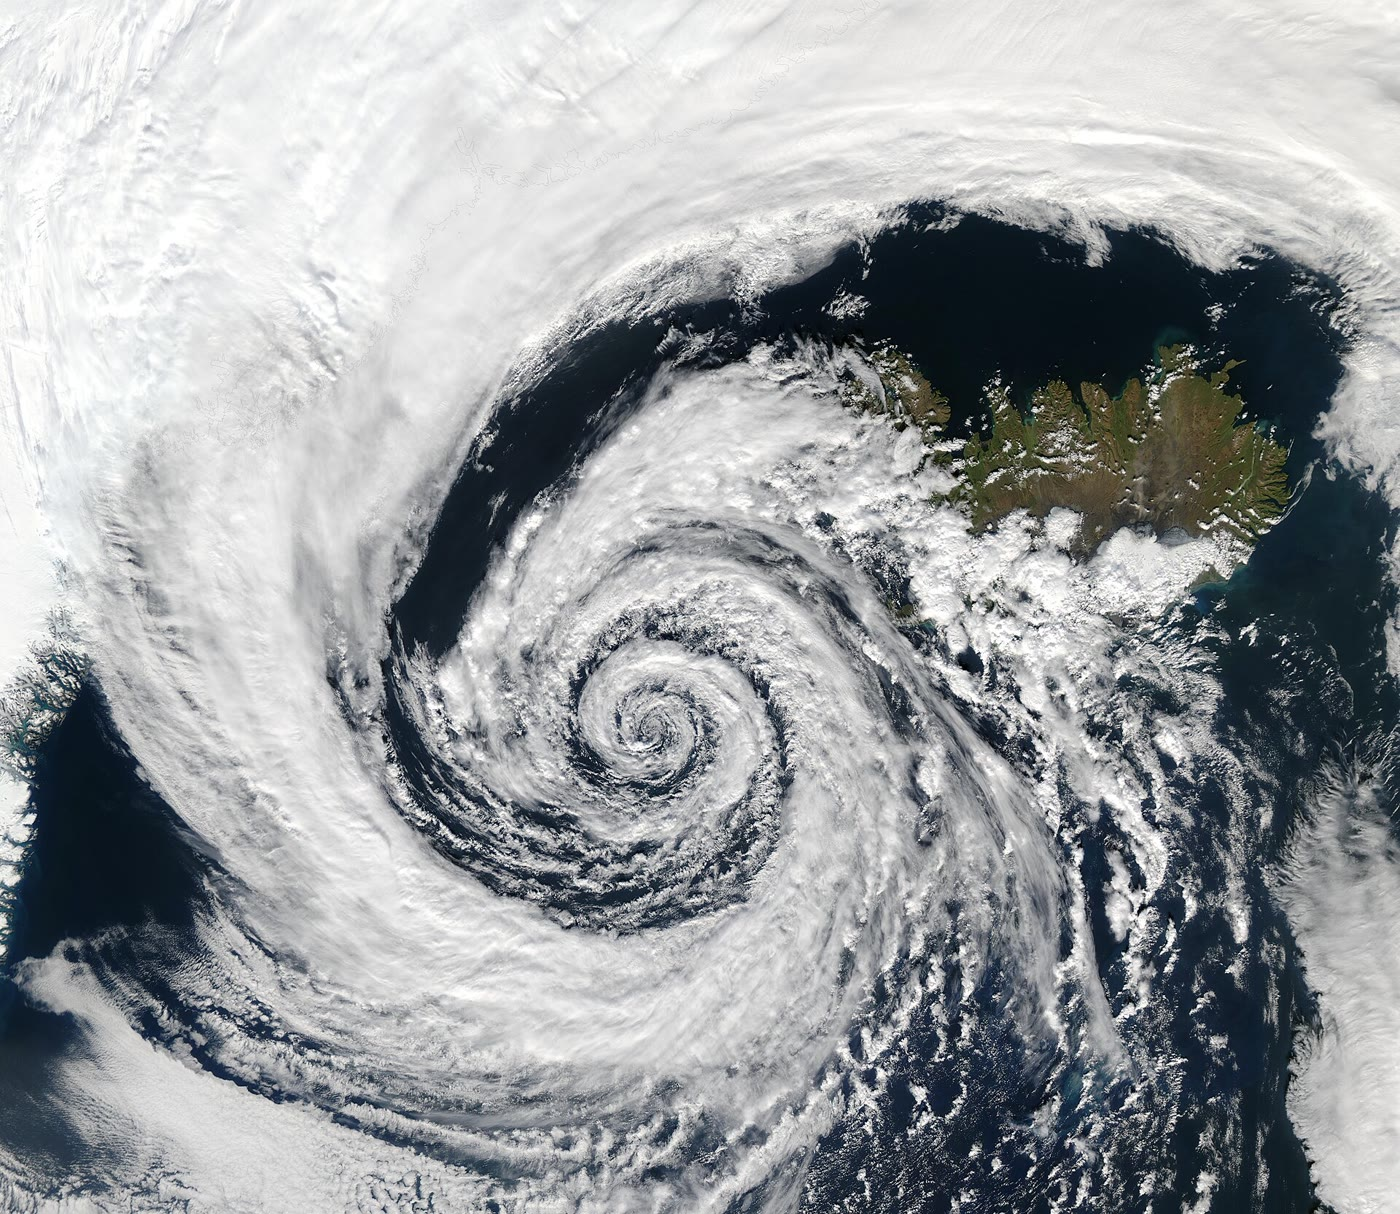
\includegraphics[width=0.58\linewidth]{images/book4/b2-22-iceland-low.jpg}
\par\smallskip{\small आइसलैंड के दक्षिण-पश्चिमी तट से दूर एक गहरा निम्न दाब, 4 सितंबर 2003, NASA के एक्वा उपग्रह के
MODIS उपकरण द्वारा देखा गया: मेघ-पट्टियाँ सर्पिल बनाती हुई केंद्र में जाती हैं। (NASA
Goddard Space Flight Center, MODIS Rapid Response Team, Jacques Descloitres, सार्वजनिक डोमेन, विकिमीडिया
कॉमन्स के माध्यम से।)}
\end{omfigure}

\section{जेट धाराएँ और रॉस्बी तरंगें}\label{sec:b2:weather-systems:rossby}

चक्रवात यादृच्छिक रूप से बिखरे नहीं होते। ध्रुवीय जेट, ध्रुवीय वाताग्र के ऊपर पछुआ पवनों का तीव्र
क्रोड, मध्य अक्षांशों के उच्च और निम्न दाब केंद्रों की स्थिति और गति के साथ चलता है; वह अपने जेट-स्ट्रीकों के अनुदिश,
उन खंडों में जहाँ उसकी पवन-गति शिखर पर होती है, सबसे तेज़ होता है, और वह ध्रुव के चारों ओर एक वलय की तरह
नहीं घूमता: वह विसर्पित होता है।
% ledger: nws4:polar-front, nws4:jet-streak

\begin{definition}[रॉस्बी तरंग; ऊपरी-स्तर द्रोणिका और कटक]\label{def:b2:weather-systems:rossby}
\emph{रॉस्बी तरंग}\index{रॉस्बी तरंग} ऊपरी क्षोभमंडल के पछुआ प्रवाह की एक तरंग है,
हज़ारों किलोमीटर लंबी द्रोणिकाओं और कटकों की एक शृंखला, जिसका उत्तर--दक्षिण आयाम बड़ा होता है।
\emph{ऊपरी-स्तर द्रोणिका}\index{ऊपरी-स्तर द्रोणिका} ऐसी तरंग में अपेक्षाकृत निम्न दाब का एक
लंबा क्षेत्र है, जहाँ प्रवाह भूमध्यरेखा की ओर मुड़ता है; \emph{ऊपरी-स्तर
कटक}\index{ऊपरी-स्तर कटक} अपेक्षाकृत उच्च दाब का एक लंबा क्षेत्र है, जहाँ वह
ध्रुव की ओर मुड़ता है।
\end{definition}
% ledger: nws4:rossby

\omterm{def:b2:weather-systems:rossby}{रॉस्बी तरंगें} इसलिए होती हैं कि कोरिऑलिस प्राचल ध्रुव की ओर बढ़ता है। ध्रुव की ओर धकेली गई वायु
बड़ा $f$ पाती है और, अपनी निरपेक्ष भ्रमिलता संरक्षित रखते हुए, भूमध्यरेखा की ओर लौट जाती है; भूमध्यरेखा की ओर
धकेली गई वायु ध्रुव की ओर लौट जाती है। वह दर जिससे $f$ उत्तर की ओर बढ़ता है,
$\beta = \mathrm{d}f/\mathrm{d}y = 2\Omega\cos\varphi/a$, जहाँ $a$ पृथ्वी की त्रिज्या है, उनकी
गति निर्धारित करती है। पुस्तक 5 (स्नातक वर्ष 3) भ्रमिलता के संरक्षण से तरंगदैर्ध्य $\lambda$ की
किसी तरंग की, एकसमान पछुआ पवन $U$ में, प्रावस्था-गति व्युत्पन्न करती है:
\[
  c = U - \frac{\beta}{k^2}, \qquad k = \frac{2\pi}{\lambda} .
\]
इसे यहाँ मान लीजिए। वायु के सापेक्ष हर \omterm{def:b2:weather-systems:rossby}{रॉस्बी तरंग} पश्चिम की ओर चलती है, और तरंग जितनी लंबी, उतनी
तेज़; पवन उसे पूर्व की ओर ले जाती है। छोटी तरंगें लगभग पवन की गति से पूर्व की ओर ले जाई जाती हैं,
लंबी तरंगें धीरे खिसकती हैं, स्थिर रहती हैं, या पश्चिम की ओर भी चलती हैं।
% ledger: earth:Trot, earth:Rmean

\begin{example}[45° उ पर तीन तरंगें]\label{ex:b2:weather-systems:rossby}
$\Omega = \qty{7.292e-5}{s^{-1}}$ (\qty{23.9345}{h} का एक नाक्षत्र दिवस) और $a =
\qty{6371}{km}$ के साथ $\beta = \qty{1.62e-11}{m^{-1}.s^{-1}}$, \ang{45} उ पर। \qty{15}{m/s} की
पछुआ पवन में \qty{4000}{km} की तरंग के लिए $\beta/k^2 = \qty{6.6}{m/s}$ है और वह
\qty{8.4}{m/s} से पूर्व की ओर चलती है; \qty{6000}{km} की तरंग के लिए $\beta/k^2 = \qty{14.8}{m/s}$ है और वह मुश्किल से चलती है,
\qty{0.2}{m/s} से; \qty{8000}{km} की तरंग \qty{11.2}{m/s} से पश्चिम की ओर चलती है।
\end{example}
% ledger: earth:Trot, earth:Rmean

लंबी तरंगों की द्रोणिकाएँ धीरे चलती हैं और देर तक टिकती हैं; उनसे होकर गुज़रने वाली छोटी तरंगें,
लघु-तरंग द्रोणिकाएँ, अपने आगे, अपनी पूर्वी ओर, उठती वायु उत्पन्न करती हैं, जहाँ सतही दाब गिरता है और
निम्न दाब विकसित होते हैं। जिस द्रोणिका का अक्ष दक्षिण-पूर्व से उत्तर-पश्चिम की ओर झुका हो, वह
प्रायः किसी विकसित होती या तीव्र होती प्रणाली का संकेत है।
% ledger: nws4:rossby

\begin{omfigure}
\centering
\begin{tikzpicture}[font=\scriptsize, >=Stealth]
\foreach \lat/\pa in {30/-72, 45/-72, 60/-108} {
  \pgfmathsetmacro{\r}{6.0*tan((90-\lat)/2)}
  \draw[black!25] (0,0) circle (\r);
  \node[black!50, fill=white, inner sep=1pt] at (\pa:\r) {\ang{\lat} उ};
}
\fill (0,0) circle (0.6mm);
\node[anchor=north, black!60] at (0,-0.08) {उत्तरी ध्रुव};
\draw[ocBlue, very thick, smooth, samples=241, domain=0:360]
  plot ({6.0*tan((90-(47+11*cos(5*\x)))/2)*cos(\x)}, {6.0*tan((90-(47+11*cos(5*\x)))/2)*sin(\x)});
\foreach \a in {18, 90, 162, 234, 306} {
  \pgfmathsetmacro{\ra}{6.0*tan((90-(47+11*cos(5*\a)))/2)}
  \pgfmathsetmacro{\rb}{6.0*tan((90-(47+11*cos(5*(\a+2))))/2)}
  \draw[ocBlue, very thick, -{Stealth[length=2.6mm]}] (\a:\ra) -- (\a+2:\rb);
}
\pgfmathsetmacro{\rt}{6.0*tan((90-36)/2)}
\node[anchor=216, ocRed!80!black, inner sep=2pt] at (36:\rt) {द्रोणिका};
\node[anchor=0, ocRed!80!black, inner sep=2pt] at (180:\rt) {द्रोणिका};
\pgfmathsetmacro{\rr}{6.0*tan((90-58)/2)}
\node[anchor=72, ocRed!80!black, inner sep=3pt] at (72:\rr) {कटक};
\end{tikzpicture}
\par\smallskip{\small उत्तरी ध्रुव के ऊपर से देखी गई जेट धारा में \omterm{def:b2:weather-systems:rossby}{रॉस्बी तरंगें} (योजनामूलक):
गोलार्ध के चारों ओर पाँच तरंगें, द्रोणिकाएँ भूमध्यरेखा की ओर और कटक ध्रुव की ओर
पहुँचते हुए। जेट पूर्व की ओर बहता है, ध्रुव के ऊपर से देखने पर वामावर्त (तीर)। अक्षांश-वृत्त
ध्रुवीय त्रिविम (स्टीरियोग्राफ़िक) मानचित्र की तरह खींचे गए हैं।}
\end{omfigure}
% ledger: nws4:rossby

कभी-कभी प्रतिरूप चलना पूरी तरह बंद कर देता है।

\begin{definition}[वायुमंडलीय अवरोधन]\label{def:b2:weather-systems:blocking}
\emph{वायुमंडलीय अवरोधन}\index{वायुमंडलीय अवरोधन} एक बड़ी, स्थायी और लगभग
स्थिर उच्च-दाब प्रणाली है, कभी-कभी किसी निम्न दाब के साथ जोड़े में, जो जेट धारा के सामान्य पूर्वमुखी
प्रवाह को बाधित करती है। अवरोधों का पता लगाने की लगभग सभी विधियाँ माँगती हैं कि वह कम से कम पाँच
दिन टिके।
\end{definition}
% ledger: wang26:blocking

अवरोध जेट और चक्रवातों को अपने चारों ओर मोड़ देता है और एक ही क्षेत्र पर दिनों तक एक ही मौसम बनाए रखता है:
अवरोध मध्य अक्षांशों में लू, सूखे, दावानल, शीत लहरें और बाढ़ लाते हैं। 2021 के जून के अंत और
जुलाई के आरंभ में एक प्रबल अवरोध से उत्तर अमेरिका के प्रशांत उत्तर-पश्चिम में लू चली,
जिससे एक हज़ार से अधिक मौतें हुईं। अवरोधन के पीछे की भौतिक
प्रक्रियाएँ अभी भी ठीक से समझी नहीं गई हैं, और संख्यात्मक मॉडल यह पुनरुत्पन्न करने में कठिनाई पाते हैं कि अवरोध
कितनी बार बनते हैं और कितनी देर टिकते हैं।
% ledger: wang26:blocking, wang26:gaps

\section{उष्णकटिबंधीय चक्रवात}\label{sec:b2:weather-systems:tropical}

उष्णकटिबंधीय चक्रवातों के पास न वाताग्र होते हैं, न पोषण के लिए तापमान का कोई अंतर। वे अपनी ऊर्जा
गर्म महासागर से, उस जल की गुप्त ऊष्मा के माध्यम से लेते हैं जिसे वे वाष्पित करते हैं, जैसा कि \cref{ch:b2:atmospheric-thermodynamics}
ने उसे मापा। छह परिस्थितियाँ उनके बनने के अनुकूल हैं: कम से कम \qty{26.5}{\celsius} का महासागरीय जल,
\qty{50}{m} की कोटि की गहराई तक; ऐसा वायुमंडल जो ऊँचाई के साथ इतनी तेज़ी से ठंडा होता हो कि
आर्द्र संवहन के लिए अस्थिर हो; लगभग \qty{5}{km} पर एक नम मध्य क्षोभमंडल; भूमध्यरेखा से
कम से कम लगभग \qty{500}{km} की दूरी, ताकि कोरिऑलिस बल निम्न दाब को संतुलन में
रख सके; सतह के निकट एक पहले से विद्यमान विक्षोभ; और दुर्बल ऊर्ध्वाधर पवन-अपरूपण, सतह और ऊपरी
क्षोभमंडल के बीच लगभग \qty{10}{m/s} से कम। ये आवश्यक हैं पर
पर्याप्त नहीं: इन्हें पूरा करने वाले अनेक विक्षोभ कभी विकसित नहीं होते।
% ledger: aoml:tc-genesis

बनने के बाद उष्णकटिबंधीय चक्रवात एक ऊष्मा इंजन है। वायु समुद्र के ऊपर लगभग
स्थिर तापमान पर सर्पिल बनाती हुई भीतर की ओर आती है, महासागर से ऊष्मा और नमी पाती हुई; आँख की दीवार में वह
रुद्धोष्म रूप से उठती है; क्षोभसीमा के निकट बहिर्वाह में वह निम्न, लगभग स्थिर तापमान पर विकिरण द्वारा
ऊष्मा खोती है; और केंद्र से दूर फिर नीचे उतरती है, इस तरह एक ऐसा चक्र पूरा करती है जो
कार्नो चक्र से मिलता-जुलता है। चक्र का कार्य समुद्र-सतह के घर्षण के विरुद्ध पवनों को
चलाता है।
% ledger: gilford21:pi

\begin{omfigure}
\centering
\begin{tikzpicture}[font=\scriptsize, >=Stealth, x=1cm, y=1cm]
% sea and axis
\fill[ocBlue!12] (0,-0.35) rectangle (12.5,0);
\draw[thick, ocBlue!70!black] (0,0) -- (12.5,0);
\node[anchor=north west, ocBlue!70!black] at (8.6,-0.02) {गर्म समुद्र, $T_s$};
\draw[dashed, black!50] (0,-0.35) -- (0,4.9);
\node[anchor=south, black!60] at (0,4.9) {केंद्र};
% eyewall cloud and outflow cloud
\fill[black!14, draw=black!40] (0.9,0.25) .. controls (0.7,1.8) and (0.75,3.3) .. (0.95,4.2)
  .. controls (3.5,4.55) and (7.0,4.45) .. (9.5,4.2) .. controls (7.0,3.9) and (3.6,3.85)
  .. (2.1,3.7) .. controls (1.95,2.6) and (1.9,1.4) .. (2.0,0.25) -- cycle;
\node[black!60] at (0.45,2.0) [rotate=90] {आँख};
\draw[black!50] (1.9,1.1) -- (2.45,1.1) node[anchor=west, black!70] {आँख की दीवार का मेघ};
% the cycle
\draw[->, very thick, ocRed] (11.4,0.3) -- (2.3,0.3);
\draw[->, very thick, ocRed] (1.45,0.45) .. controls (1.4,1.6) and (1.45,3.0) .. (1.75,4.0);
\draw[->, very thick, ocBlue] (2.2,4.25) -- (11.2,4.25);
\draw[->, very thick, ocBlue] (11.6,4.05) .. controls (11.75,2.8) and (11.75,1.5) .. (11.6,0.45);
\fill (11.6,0.3) circle (0.7mm) node[right=2pt] {A};
\fill (1.45,0.3) circle (0.7mm) node[left=2pt] {B};
\fill (1.8,4.25) circle (0.7mm) node[above left=1pt] {C};
\fill (11.6,4.25) circle (0.7mm) node[above right=1pt] {D};
\node[anchor=south, align=center] at (6.5,0.35) {A$\to$B: समुद्र के ऊपर लगभग $T_s$ पर अंतर्वाह,
  ऊष्मा और नमी लेते हुए};
\node[anchor=west, align=left] at (2.25,2.3) {B$\to$C: आँख की दीवार में उठती है,\\ऊष्मा का
  विनिमय किए बिना (आर्द्र रुद्धोष्म वक्र)};
\node[anchor=south, align=center] at (6.5,4.62) {C$\to$D: क्षोभसीमा के निकट लगभग
  $T_o$ पर बहिर्वाह, विकिरण द्वारा ऊष्मा खोते हुए};
\node[anchor=east, align=right] at (11.45,2.3) {D$\to$A: केंद्र से\\दूर नीचे उतरती है};
\end{tikzpicture}
\par\smallskip{\small उष्णकटिबंधीय चक्रवात का ऊष्मा इंजन, केंद्र से बाहर की ओर एक ऊर्ध्वाधर काट
(योजनामूलक, पैमाने के बिना): ऊष्मा समुद्र-सतह के तापमान पर ली जाती है
(A$\to$B) और बहिर्वाह के बहुत कम तापमान पर छोड़ी जाती है (C$\to$D), जैसे किसी कार्नो
चक्र में।}
\end{omfigure}
% ledger: gilford21:pi

\begin{proposition}[संभाव्य तीव्रता]\label{prop:b2:weather-systems:pi}
\index{संभाव्य तीव्रता}
किसी उष्णकटिबंधीय चक्रवात की \emph{\omterm{prop:b2:weather-systems:pi}{संभाव्य तीव्रता}}, सतह के निकट वह अधिकतम पवन-गति जिसे
उसके चारों ओर का महासागर और वायुमंडल बनाए रख सकते हैं, लगभग इससे दी जाती है:
\[
  V_{\max}^2 = \frac{C_k}{C_D}\,\frac{T_s - T_o}{T_o}\,\bigl(h_o^* - h^*\bigr),
\]
जहाँ $T_s$ समुद्र-सतह का तापमान है, $T_o$ बहिर्वाह का तापमान, $C_k/C_D$
समुद्र और वायु के बीच एन्थैल्पी और संवेग के विनिमय गुणांकों का अनुपात, जो
सामान्यतः 0.9 लिया जाता है, और $h_o^* - h^*$ समुद्र-सतह पर संतृप्ति पर $c_pT + gz + Lq$ का,
परिसीमा परत के ऊपर की वायु में उसके संतृप्ति मान पर आधिक्य (स्वीकृत)।
\end{proposition}
% ledger: gilford21:pi

भिन्न $(T_s - T_o)/T_o$ भौतिकी की पुस्तकों की कार्नो दक्षता $(T_s - T_o)/T_s$ नहीं है: वह
गुणक $T_s/T_o$ से बड़ा है, क्योंकि कार्य को क्षयित करने वाला घर्षण समुद्र-सतह के निकट
भीतर आती वायु को गर्म करता है, और वह ऊष्मा इंजन द्वारा फिर से उपयोग होती है। अंतिम
गुणक ईंधन है। ऐसे उष्णकटिबंधीय वायुमंडल में जिसका तापमान अपनी परिसीमा-परत वायु के \omterm{def:b2:atmospheric-thermodynamics:moist-adiabat}{आर्द्र रुद्धोष्म वक्र} का
अनुसरण करता है, $h^*$ उस वायु में $c_pT + gz + Lq$ का मान है, और $h_o^* - h^*$
मापता है कि समुद्र के ऊपर की वायु समुद्र के तापमान पर संतृप्ति से कितनी दूर है:
\[
  h_o^* - h^* \approx c_p\,(T_s - T_a) + L\,(q_s^* - q_a),
\]
जहाँ $T_a$ और $q_a$ सतह के निकट वायु का तापमान और \omterm{def:b2:atmospheric-thermodynamics:moist-air}{विशिष्ट आर्द्रता} हैं और
$q_s^*$ समुद्र-सतह के तापमान पर संतृप्त \omterm{def:b2:atmospheric-thermodynamics:moist-air}{विशिष्ट आर्द्रता}।
% ledger: gilford21:pi

\begin{example}[एक संभाव्य तीव्रता]\label{ex:b2:weather-systems:pi}
\qty{29}{\celsius} के समुद्र के ऊपर \qty{1015}{hPa} पर वायु \qty{28}{\celsius} पर है,
\qty{80}{\percent} की सापेक्ष आर्द्रता के साथ, और बहिर्वाह \qty{200}{K} पर है, जो गर्म उष्णकटिबंधीय महासागरों
के ऊपर एक प्रतिनिधि वार्षिक माध्य है। \cref{prop:b2:atmospheric-thermodynamics:es,prop:b2:atmospheric-thermodynamics:humidity} से,
$e_s(\qty{29}{\celsius}) = \qty{41.0}{hPa}$, अतः $q_s^* = \qty{25.5}{g/kg}$, और वायु का,
$e = 0.8 \times \qty{38.7}{hPa}$ के साथ, $q_a = \qty{19.2}{g/kg}$ है। तब $h_o^* - h^* = 1004.5 \times
1 + 2.501 \times 10^6 \times 0.0063 = \qty{16.8}{kJ/kg}$, गुणक $(T_s - T_o)/T_o$
$(302.15 - 200)/200 = 0.511$ है, और $V_{\max} = \sqrt{0.9 \times 0.511 \times 16\,800} =
\qty{88}{m/s}$।
\end{example}
% ledger: gilford21:pi

सबसे प्रबल तूफ़ान ऐसे मानों के निकट पहुँचते हैं: सैफ़िर--सिम्पसन पैमाने का शीर्ष, श्रेणी
5, \qty{70}{m/s} से आरंभ होता है, और हाल के पाँच तूफ़ान \qty{86}{m/s} से आगे गए हैं। अधिकांश तूफ़ान
शायद ही कभी अपनी \omterm{prop:b2:weather-systems:pi}{संभाव्य तीव्रता} तक पहुँचते हैं: वास्तविक तूफ़ान विरले ही उस स्थायी अवस्था में होते हैं जो
सिद्धांत मानता है, और सिद्धांत ऊर्ध्वाधर पवन-अपरूपण, तूफ़ान में खींची गई शुष्क वायु और उसके चारों ओर की
वायु के नीचे उतरने को छोड़ देता है, जो तूफ़ान को दुर्बल करते हैं।
% ledger: wk24:scale, gilford21:limits, aoml:tc-weaken

\begin{omfigure}
\centering
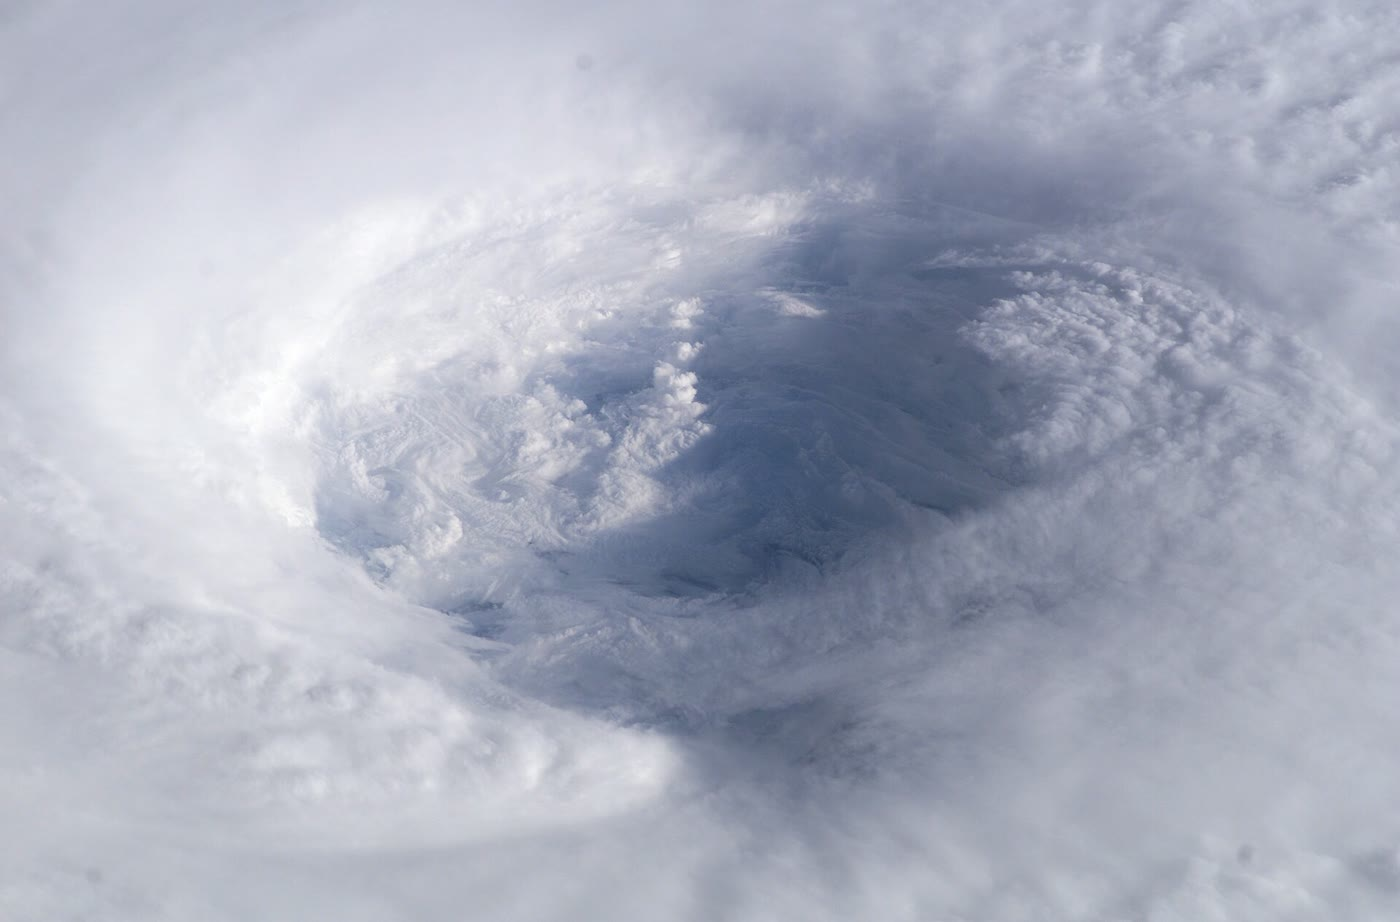
\includegraphics[width=0.62\linewidth]{images/book4/b2-22-isabel-eye.jpg}
\par\smallskip{\small हरिकेन इज़ाबेल की आँख, 13 सितंबर 2003, अंतरराष्ट्रीय
अंतरिक्ष स्टेशन से खींचा गया फ़ोटो: आँख की दीवार किसी स्टेडियम की तरह आँख के निचले मेघों तक उतरती है।
(NASA astronaut Ed Lu, सार्वजनिक डोमेन, विकिमीडिया कॉमन्स के माध्यम से।)}
\end{omfigure}

\section{संख्यात्मक मौसम पूर्वानुमान}\label{sec:b2:weather-systems:nwp}

\begin{definition}[संख्यात्मक मौसम पूर्वानुमान; आँकड़ा समावेशन; समष्टि पूर्वानुमान; पूर्वानुमेयता सीमा]\label{def:b2:weather-systems:nwp}
\emph{संख्यात्मक मौसम पूर्वानुमान}\index{संख्यात्मक मौसम पूर्वानुमान} कंप्यूटर द्वारा
पूर्वानुमान है: वायुमंडल की गति, ऊर्जा और जल को नियंत्रित करने वाले समीकरणों का उसकी प्रेक्षित अवस्था से
समय में आगे समाकलन किया जाता है। \emph{आँकड़ा समावेशन}\index{आँकड़ा समावेशन}
नवीनतम प्रेक्षणों को पहले के प्रेक्षणों से बने एक अल्प-अवधि पूर्वानुमान के साथ मिलाकर
वर्तमान अवस्था का सर्वोत्तम अनुमान, यानी विश्लेषण, प्राप्त करता है, जिससे
पूर्वानुमान आरंभ होता है। \emph{समष्टि पूर्वानुमान}\index{समष्टि पूर्वानुमान} पूर्वानुमानों का एक समूह है जो
थोड़ी भिन्न आरंभिक अवस्थाओं से, और मॉडल के थोड़े भिन्न संस्करणों के साथ, चलाया जाता है, ताकि
संभव मौसम का परास और उसकी संभाविता दिखे। \emph{पूर्वानुमेयता
सीमा}\index{पूर्वानुमेयता सीमा} वह समय है जिसके बाद मौसम की अवस्था का पूर्वानुमान
जलवायु से लगाए गए अनुमान से बेहतर नहीं रहता, क्योंकि आरंभिक अवस्था की त्रुटियाँ
वायुमंडल की किन्हीं दो अवस्थाओं के बीच के अंतरों जितनी बड़ी हो चुकी होती हैं।
\end{definition}
% ledger: nws4:nwp, ecmwf4:da, ecmwf4:ens-fs, krish19:predictability

पहला संख्यात्मक पूर्वानुमान 1950 में ENIAC पर परिकलित किया गया, जो पहले इलेक्ट्रॉनिक
कंप्यूटरों में से एक था। आज एक वैश्विक मॉडल वायुमंडल को कुछ किलोमीटर चौड़ी कोशिकाओं के एक ग्रिड में बाँटता है
और ऐसे विश्लेषण से आरंभ होता है जो मौसम-वेधशालाओं, विमानों,
रेडियोसॉन्डों, जहाज़ों, प्लवों और, सबसे बढ़कर, उपग्रहों के प्रेक्षणों को मिलाता है, जो वैश्विक पूर्वानुमानों की
कुशलता में सबसे बड़ा योगदान देते हैं। एक बड़े पूर्वानुमान केंद्र पर समष्टि
में 51 सदस्य होते हैं, एक नियंत्रण रन और 50 विक्षुब्ध रन, लगभग \qty{9}{km} के विभेदन पर, जो
दिन में दो बार 15 दिन आगे तक चलाए जाते हैं।
% ledger: krish19:predictability, ecmwf4:da, ecmwf4:ens

सर्वोत्तम विश्लेषण से आरंभ हो सकने वाले पूर्वानुमान को विक्षुब्ध क्यों करें? क्योंकि वायुमंडल
अराजक है, अपनी आरंभिक अवस्था के प्रति संवेदनशील। 1963 में प्रकाशित तीन चरों का एक निकाय इसे
सबसे छोटे पैमाने पर दिखाता है।

\begin{proposition}[लॉरेंज़ निकाय]\label{prop:b2:weather-systems:lorenz}
निकाय
\[
  \dot x = \sigma(y - x), \qquad \dot y = x(r - z) - y, \qquad \dot z = xy - bz,
\]
$\sigma = 10$, $r = 28$ और $b = 8/3$ के साथ, निम्नलिखित गुण रखता है।
\begin{enumerate}
  \item उसके स्थिर बिंदु मूलबिंदु और $C_\pm = \bigl(\pm\sqrt{b(r - 1)}, \pm\sqrt{b(r - 1)},
        r - 1\bigr) = (\pm 8.49, \pm 8.49, 27)$ हैं।
  \item उसके प्रावस्था-अवकाश में हर आयतन $\mathrm{e}^{-(\sigma + 1 + b)t}$ की तरह सिकुड़ता है: उसके
        प्रक्षेप-पथ शून्य आयतन के एक समुच्चय पर समाप्त होते हैं, आकर्षक पर।
  \item आकर्षक पर, एक छोटी दूरी $\delta_0$ से आरंभ होने वाले दो प्रक्षेप-पथ
        औसतन $\delta(t) \approx \delta_0\,\mathrm{e}^{\lambda t}$ की तरह अलग होते हैं, जहाँ $\lambda =
        0.906$, जब तक $\delta$ आकर्षक के आकार तक न पहुँच जाए (परिकलित, स्वीकृत)। छोटी
        त्रुटियाँ हर $\ln 2/\lambda = 0.77$ समय-इकाई में दोगुनी होती हैं।
\end{enumerate}
\end{proposition}
% ledger: nolitia22:lorenz

\begin{proof}[1 और 2 का प्रमाण]
किसी स्थिर बिंदु पर पहले समीकरण से $y = x$; तीसरा $z = x^2/b$ देता है; दूसरा
$x(r - 1 - x^2/b) = 0$ बन जाता है, अतः $x = 0$ या $x^2 = b(r - 1) = 72$। सदिश क्षेत्र का
अपसरण $\partial_x\dot x + \partial_y\dot y + \partial_z\dot z = -\sigma - 1 - b$ है, एक
नियतांक, और अपसरण प्रमेय से प्रवाह के साथ बहता आयतन $V$ इसका पालन करता है: $\dot V =
-(\sigma + 1 + b)V$।
\end{proof}

आकृतियाँ दिखाती हैं कि प्रस्ताव का क्या अर्थ है। \num{e-5} की दूरी पर आरंभ होने वाले दो रन लगभग
पंद्रह समय-इकाइयों तक एक-दूसरे का अनुसरण करते हैं, फिर हमेशा के लिए अलग हो जाते हैं: हर एक अब भी निकाय का
एक संभाव्य प्रक्षेप-पथ लगता है, पर वे अब एक ही प्रक्षेप-पथ नहीं हैं। \num{e-8} की दूरी पर आरंभ किए गए
200 रन-जोड़ों पर औसत लेने पर दूरी दर $\lambda$ से चरघातांकी रूप से बढ़ती है, लघुगणकीय पैमाने पर एक सीधी
रेखा, जब तक वह आकर्षक के आकार पर संतृप्त न हो जाए। आरंभिक त्रुटि जो भी हो, वह उस आकार तक
पहुँचती है: छोटी आरंभिक त्रुटि केवल उस क्षण को टालती है, हर दस गुना कमी के लिए
$\ln 10/\lambda = 2.5$ समय-इकाई से।
% ledger: nolitia22:lorenz

\begin{omfigure}
\centering
% figdata/bachelor-2/weather.py parts traj, butterfly
\begin{tikzpicture}
\begin{groupplot}[group style={group size=2 by 1, horizontal sep=1.5cm},
  tick label style={font=\scriptsize}, label style={font=\small}]
\nextgroupplot[width=0.58\linewidth, height=5.0cm, xmin=0, xmax=30, ymin=-22, ymax=22,
  xlabel={समय}, ylabel={$x$}, legend style={font=\scriptsize, at={(0.5,1.02)},
  anchor=south, draw=none, legend columns=2, /tikz/every even column/.append style={column
  sep=0.4cm}}, legend cell align=left]
\addplot[ocBlue, thin] table[x=t, y=x1] {figdata/out/bachelor-2-weather-traj.dat};
\addlegendentry{रन 1}
\addplot[ocRed, thin, densely dashed] table[x=t, y=x2] {figdata/out/bachelor-2-weather-traj.dat};
\addlegendentry{रन 2, \num{e-5} दूर से आरंभ}
\nextgroupplot[width=0.4\linewidth, height=5.0cm, xmin=-22, xmax=22, ymin=0, ymax=52,
  xlabel={$x$}, ylabel={$z$}]
\addplot[black!70, very thin] table[x=x, y=z] {figdata/out/bachelor-2-weather-butterfly.dat};
\addplot[only marks, mark=*, mark size=1.3pt, ocRed] coordinates {(8.485,27) (-8.485,27)};
\end{groupplot}
\end{tikzpicture}
\par\smallskip{\small लॉरेंज़ निकाय ($\sigma = 10$, $r = 28$, $b = 8/3$), 0.01 के समय-चरण के साथ
रुंगे--कुट्टा विधि से समाकलित। बाएँ: दो रन जो \num{e-5} की दूरी से, $x$ में,
आकर्षक पर आरंभ होते हैं। दाएँ: 40 समय-इकाइयों का एक रन, $y$ के अनुदिश देखा गया, स्थिर बिंदुओं
$C_\pm$ (लाल) के साथ।}
\end{omfigure}
% ledger: nolitia22:lorenz

\begin{omfigure}
\centering
% figdata/bachelor-2/weather.py part growth
\begin{tikzpicture}
\begin{axis}[width=0.72\linewidth, height=5.6cm, xmin=0, xmax=30, ymode=log, ymin=1e-9,
  ymax=1e3, ytick={1e-9,1e-7,1e-5,1e-3,1e-1,1e1,1e3}, xlabel={समय}, ylabel={रनों के बीच दूरी}, tick label style={font=\scriptsize},
  label style={font=\small}, legend style={font=\scriptsize, at={(0.02,0.98)}, anchor=north west,
  draw=none, fill=none}, legend cell align=left, unbounded coords=discard, grid=major,
  grid style={black!8}]
\addplot[ocBlue, line width=1.6pt, opacity=0.55] table[x=t, y expr=10^\thisrow{log10d}]
  {figdata/out/bachelor-2-weather-growth.dat};
\addlegendentry{200 जोड़ों का माध्य (ज्यामितीय)}
\addplot[black, densely dashed, thin] table[x=t, y expr=10^\thisrow{fit}]
  {figdata/out/bachelor-2-weather-growth.dat};
\addlegendentry{फ़िट किया गया चरघातांकी, $t = 2$ से 16}
\end{axis}
\end{tikzpicture}
\par\smallskip{\small लॉरेंज़ निकाय के उन रन-जोड़ों के बीच की दूरी की वृद्धि जो
\num{e-8} की दूरी पर आरंभ किए गए। फ़िट की गई रेखा हर 2.57 समय-इकाई में दस गुना बढ़ती है, 0.897 की दर;
सबसे बड़ा ल्यापुनोव घातांक, एक ही जोड़े को 2000 समय-इकाइयों तक पुनःप्रसामान्यीकृत करके परिकलित,
0.909 है, जबकि प्रकाशित मान 0.906 है। वृद्धि आकर्षक के आकार पर रुक जाती है।}
\end{omfigure}
% ledger: nolitia22:lorenz

वायुमंडल भी इसी तरह व्यवहार करता है, बहुत अधिक चरों के साथ और ऐसी त्रुटियों के साथ जो
भिन्न पैमानों पर भिन्न दरों से बढ़ती हैं। 1980 के दशक के पूर्वानुमानों से पाया गया कि छोटी त्रुटियाँ
लगभग 2.4 दिनों में दोगुनी होती हैं, और मौसम की अवस्था का विश्वसनीय पूर्वानुमान लगभग दस दिनों से
पहले ही रुक जाता है। ऐसे प्रयोग जो आज की आरंभिक अवस्था की अनिश्चितता को घटाते हैं, मॉडल को
पूर्ण मानकर, पाते हैं कि पूर्ण आरंभिक परिस्थितियाँ केवल चार से पाँच दिन जोड़ेंगी, और
कि 90 प्रतिशत की कमी लगभग पूरा लाभ पहले ही दे देती है: त्रुटियाँ जितनी छोटी होती हैं, उतनी ही तेज़ी से बढ़ती हैं,
संवहन में गुप्त ऊष्मा के मुक्त होने के माध्यम से, उन पैमानों पर जो पूर्वानुमान द्वारा विभेदित पैमानों से छोटे हैं।
मध्य अक्षांशों की \omterm{def:b2:weather-systems:nwp}{पूर्वानुमेयता सीमा} लगभग दो सप्ताह पर है। पूर्वानुमान
प्रति दशक लगभग एक दिन पाते हैं क्योंकि बेहतर प्रेक्षण, समावेशन और मॉडल उन्हें उस सीमा के
अधिक निकट ले जाते हैं; वे उसे पार नहीं कर सकते।
% ledger: krish19:predictability, selz22:limit, bauer:day-per-decade

समष्टि इसे एक उपकरण में बदल देती है। उसके सदस्य ऐसे विश्लेषणों से आरंभ होते हैं जो लगभग उतने ही भिन्न होते हैं
जितना विश्लेषण स्वयं अनिश्चित है; जब तक वे सहमत रहते हैं, पूर्वानुमान स्पष्ट होता है; जब वे
फैलते हैं, तो पूर्वानुमान को यह कहना चाहिए, और वह प्रायिकताएँ देता है। किसी पूर्वानुमान को विश्वसनीय कहते हैं जब
वे घटनाएँ जिनकी वह \qty{70}{\percent} प्रायिकता से घोषणा करता है, \qty{70}{\percent}
मामलों में घटित होती हैं।
% ledger: ecmwf4:ens-fs

\begin{inthelab}[एक पूर्वानुमान केंद्र पर एक दिन]
\begin{minipage}[t]{0.54\linewidth}\vspace{0pt}
किसी वैश्विक पूर्वानुमान केंद्र पर दिन दो समयों, 00 और 12 UTC, के इर्द-गिर्द घूमता है। हर समय के आसपास मान्य
प्रेक्षण लाखों की संख्या में आते हैं, उपग्रहों, रेडियोसॉन्डों, विमानों, जहाज़ों,
प्लवों और मौसम-वेधशालाओं से; \omterm{def:b2:weather-systems:nwp}{आँकड़ा समावेशन} उन्हें पिछले अल्प पूर्वानुमान के साथ मिलाकर
विश्लेषण बनाता है। मॉडल उससे आरंभ होते हैं, समष्टि भी, और पूर्वानुमान अपने उपयोगकर्ताओं तक
कई घंटे बाद पहुँचते हैं, जब सुपरकंप्यूटर 15 दिन आगे तक चल चुके होते हैं। फिर पूर्वानुमानकर्ता
रनों की तुलना करते हैं, उन्हें नवीनतम प्रेक्षणों और उपग्रह चित्रों से जाँचते हैं,
चक्रवातों और वाताग्रों का अनुसरण करते हैं, और समष्टि की प्रायिकताओं को चेतावनियों और
पूर्वानुमानों में बदलते हैं।
\end{minipage}\hfill
\begin{minipage}[t]{0.42\linewidth}\vspace{0pt}
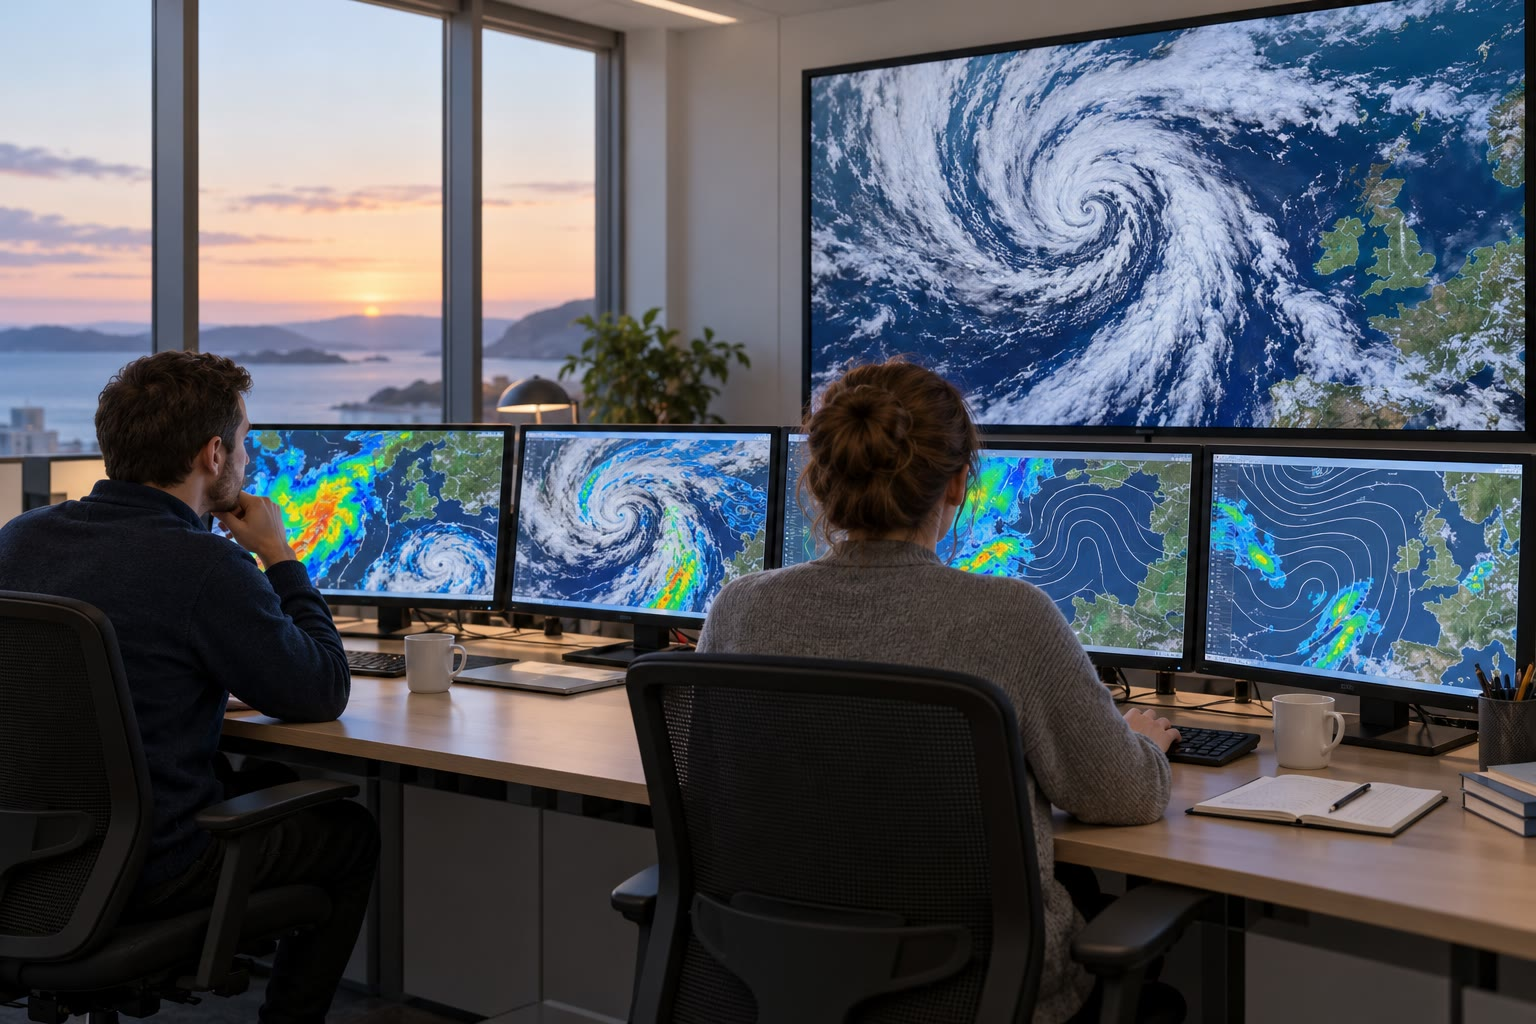
\includegraphics[width=\linewidth]{images/book4/ai/b2-forecast-office.jpg}

{\scriptsize उपग्रह चित्रों और मॉडल चार्टों के सामने काम करते पूर्वानुमानकर्ता
(AI से बनाया गया चित्रण)।}
\end{minipage}
% ledger: ecmwf4:ens, ecmwf4:da, mo:how-forecasts
\end{inthelab}

\section*{अभ्यास}\label{sec:b2:weather-systems:exercises}

अभ्यासों के आँकड़े, अन्यथा न कहा जाए तो: $\Omega = \qty{7.292e-5}{s^{-1}}$, $a =
\qty{6371}{km}$, $g = \qty{9.81}{m.s^{-2}}$, $c_p = \qty{1004.5}{J.kg^{-1}.K^{-1}}$, $L =
\qty{2.501e6}{J/kg}$, और \cref{ch:b2:atmospheric-thermodynamics} के अभ्यासों का
संतृप्त \omterm{def:b2:atmospheric-thermodynamics:moist-air}{वाष्प दाब}।
% ledger: earth:Trot, earth:Rmean

\begin{exercise}[$\star$]\label{exo:b2:weather-systems:1}
\ang{50} उ पर एक शीत वाताग्र \qty{275}{K} की वायु को \qty{281}{K} की वायु से अलग करता है, और उसके अनुदिश
पवन \qty{15}{m/s} बदलती है। (क)~$f$ की गणना कीजिए। (ख)~\omterm{def:b2:weather-systems:fronts}{वाताग्र-पृष्ठ} की ढलान की गणना कीजिए,
$N$ में 1 के रूप में। (ग)~भूमि पर वाताग्र के कितना पीछे \omterm{def:b2:weather-systems:fronts}{वाताग्र-पृष्ठ}
\qty{1}{km} तक पहुँचता है? (घ)~यदि उसी पवन-परिवर्तन पर तापमान-अंतर
दोगुना हो जाए तो ढलान का क्या होता है?
\end{exercise}

\begin{exercise}[$\star$]\label{exo:b2:weather-systems:2}
एक उष्ण \omterm{def:b2:weather-systems:fronts}{वाताग्र-पृष्ठ} 150 में 1 की ढलान से उठता है और \qty{25}{km/h} से चलता है। (क)~भूमि पर
वाताग्र से कितना आगे \omterm{def:b2:weather-systems:fronts}{वाताग्र-पृष्ठ} \qty{6}{km} ऊपर है? (ख)~एक प्रेक्षक वहाँ उस पर ऊँचे मेघ बनते
देखता है। कितने समय बाद वाताग्र प्रेक्षक तक पहुँचता है? (ग)~इस बीच प्रेक्षक जो मेघ-क्रम देखता है,
उसका वर्णन कीजिए।
\end{exercise}
% ledger: ucar:warm-front

\begin{exercise}[$\star$]\label{exo:b2:weather-systems:3}
उत्तरी गोलार्ध के एक मानचित्र पर (क)~अपनी दक्षिण-पूर्वी ओर नीले त्रिभुजों वाली एक रेखा एक निम्न दाब से
दक्षिण-पश्चिम की ओर जाती है; (ख)~अपनी उत्तरी ओर लाल अर्धवृत्तों वाली एक रेखा उसी निम्न दाब से पूर्व की ओर जाती है;
(ग)~दोनों प्रतीकों वाली एक बैंगनी रेखा किसी दूसरे निम्न दाब से उस बिंदु तक जाती है जहाँ दो अन्य वाताग्र शुरू होते हैं;
(घ)~एक रेखा पर बारी-बारी से दक्षिणी ओर नीले त्रिभुज और उत्तरी ओर लाल अर्धवृत्त हैं।
हर वाताग्र का नाम बताइए, कहिए कि ठंडी वायु कहाँ है और हर एक किस ओर चलता है।
\end{exercise}
% ledger: ucar4:stationary-occluded, nws4:occluded

\begin{exercise}[$\star$]\label{exo:b2:weather-systems:4}
\ang{45} उ पर \qty{12}{m/s} की पछुआ पवन में: (क)~$\beta$ की गणना कीजिए। (ख)~\qty{4000}{km} और \qty{8000}{km}
की तरंगों की प्रावस्था-गति की गणना कीजिए। (ग)~हर एक किस ओर चलती है, और एक दिन में
कितनी दूर?
\end{exercise}

\begin{exercise}[$\star\star$]\label{exo:b2:weather-systems:5}
(क)~दिखाइए कि पछुआ पवन $U$ में \omterm{def:b2:weather-systems:rossby}{रॉस्बी तरंग} तब स्थिर रहती है जब $\lambda = 2\pi\sqrt{U/\beta}$।
(ख)~इसकी गणना \ang{45} उ पर $U = \qty{12}{m/s}$ के लिए कीजिए। (ग)~ऐसी कितनी तरंगें
अक्षांश-वृत्त के चारों ओर समाती हैं? (घ)~अधिक प्रबल पछुआ पवन कम संख्या की, लंबी स्थिर तरंगों के अनुकूल क्यों होगी?
\end{exercise}

\begin{exercise}[$\star\star$]\label{exo:b2:weather-systems:6}
लॉरेंज़ निकाय के लिए: (क)~$C_+$ पर तीनों अवकलजों की गणना करके जाँचिए कि वह एक स्थिर बिंदु है।
(ख)~प्रावस्था-अवकाश का एक छोटा आयतन एक समय-इकाई में किस गुणक से सिकुड़ता है? (ग)~यह दो निकटवर्ती
प्रक्षेप-पथों को अलग होने से क्यों नहीं रोकता?
\end{exercise}

\begin{exercise}[$\star\star$]\label{exo:b2:weather-systems:7}
लॉरेंज़ निकाय के लिए $\lambda = 0.906$ और आकार 10 का एक आकर्षक लीजिए। (क)~छोटी त्रुटियों के
दोगुना-काल की गणना कीजिए। (ख)~\num{e-8} की त्रुटि को आकर्षक के आकार तक पहुँचने में कितना समय लगता है?
(ग)~हज़ार गुना छोटी आरंभिक त्रुटि उस क्षण को कितना टालती है? वह (ख) में पाए गए समय का
कौन-सा भाग है?
\end{exercise}
% ledger: nolitia22:lorenz

\begin{exercise}[$\star\star$]\label{exo:b2:weather-systems:8}
\qty{303}{K} के समुद्र का बहिर्वाह \qty{195}{K} पर है; असाम्य $h_o^* - h^* =
\qty{15}{kJ/kg}$ है और $C_k/C_D = 0.9$। (क)~\omterm{prop:b2:weather-systems:pi}{संभाव्य तीव्रता} की गणना कीजिए। (ख)~इसकी तुलना
श्रेणी 5 की देहली से और हाल के सबसे तेज़ तूफ़ानों से कीजिए। (ग)~अधिकांश तूफ़ान उस तक
क्यों नहीं पहुँचते?
\end{exercise}
% ledger: gilford21:pi, wk24:scale

\begin{exercise}[$\star\star$]\label{exo:b2:weather-systems:9}
\cref{exo:b2:weather-systems:8} के तूफ़ान के लिए: (क)~समुद्र-सतह और बहिर्वाह के बीच काम करने वाले
इंजन की कार्नो दक्षता की गणना कीजिए। (ख)~\cref{prop:b2:weather-systems:pi} का गुणक $(T_s - T_o)/T_o$
और दोनों का अनुपात परिकलित कीजिए। (ग)~अंतर समझाइए।
\end{exercise}
% ledger: gilford21:pi

\begin{exercise}[$\star\star\star$]\label{exo:b2:weather-systems:10}
(क)~घनत्वों को सटीक रखते हुए \cref{prop:b2:weather-systems:slope} को फिर से व्युत्पन्न कीजिए, और दिखाइए कि
ठंडी वायु को नीचे ही होना चाहिए। (ख)~\qty{50}{km} चौड़े, \ang{45} उ पर स्थित एक वाताग्र क्षेत्र के आर-पार
वाताग्र के अनुदिश पवन \qty{10}{m/s} बदलती है। क्षेत्र की आपेक्षिक भ्रमिलता की गणना कीजिए और उसकी तुलना
$f$ से कीजिए। (ग)~क्षेत्र चक्रवाती है या प्रतिचक्रवाती?
\end{exercise}

\begin{exercise}[$\star\star\star$]\label{exo:b2:weather-systems:11}
मान लीजिए पूर्वानुमान की त्रुटियाँ हर 2.4 दिनों में दोगुनी होती हैं, \qty{0.5}{K} से आरंभ होती हैं और
\qty{6}{K} पर बेकार हो जाती हैं। (क)~उपयोगी पूर्वानुमानों का क्षितिज ज्ञात कीजिए। (ख)~यदि मॉडल पूर्ण होता, तो प्रति
दशक एक दिन पाने के लिए आरंभिक त्रुटि को हर दशक किस गुणक से घटना होगा? (ग)~प्रयोग पाते हैं कि
दस गुना छोटी आरंभिक त्रुटि केवल 4 से 5 दिन जोड़ती है। यह छोटी त्रुटियों के लिए किस दोगुना-काल का संकेत देता है,
और यह छोटी त्रुटियों के बढ़ने के बारे में क्या कहता है?
\end{exercise}
% ledger: krish19:predictability, selz22:limit, bauer:day-per-decade

\begin{exercise}[$\star\star\star$]\label{exo:b2:weather-systems:12}
\cref{ex:b2:weather-systems:pi} लीजिए और समुद्र और वायु दोनों को \qty{1}{K} गर्म कीजिए, जबकि
सापेक्ष आर्द्रता और बहिर्वाह का तापमान अपरिवर्तित रहें। (क)~$q_s^*$, $q_a$ और
असाम्य फिर से परिकलित कीजिए। (ख)~\omterm{prop:b2:weather-systems:pi}{संभाव्य तीव्रता} फिर से परिकलित कीजिए। (ग)~वह प्रति केल्विन कितने प्रतिशत
बढ़ती है, और कौन-सा गुणक सबसे अधिक योगदान देता है?
\end{exercise}
% ledger: gilford21:pi

\begin{problem}[{सप्ताहांत समस्या --- कितना आगे?}]\label{pb:b2:weather-systems:1}
\ang{50} उ पर एक काल्पनिक मौसम चार्ट एक शीत वाताग्र को एक कस्बे की ओर बढ़ता हुआ दिखाता है, और ऊपर जेट धारा में
एक \omterm{def:b2:weather-systems:rossby}{रॉस्बी तरंग}। समस्या पहले वाताग्र का, फिर तरंग का अनुसरण करती है, फिर पूछती है कि इनमें से कुछ भी
कितना आगे तक पूर्वानुमानित किया जा सकता है। अभ्यासों के आँकड़ों का उपयोग कीजिए।

\medskip\noindent\textbf{भाग I --- वाताग्र।}
06 UTC पर शीत वाताग्र कस्बे से \qty{480}{km} पश्चिम में है, 12 UTC पर \qty{390}{km}। उसके पीछे
वायु \qty{277}{K} पर है, उष्ण खंड में \qty{285}{K} पर, और वाताग्र के अनुदिश पवन
उसके आर-पार \qty{16}{m/s} बदलती है।
\begin{enumerate}
  \item वाताग्र की गति ज्ञात कीजिए।
  \item वह किस समय कस्बे तक पहुँचता है?
  \item $f$ की गणना \ang{50} उ पर कीजिए।
  \item \omterm{def:b2:weather-systems:fronts}{वाताग्र-पृष्ठ} की ढलान की गणना कीजिए।
  \item वाताग्र के गुज़रने के छह घंटे बाद कस्बे के ऊपर \omterm{def:b2:weather-systems:fronts}{वाताग्र-पृष्ठ} कितना ऊँचा है?
  \item गुज़रने के कितने समय बाद ठंडी वायु कस्बे के ऊपर \qty{1.5}{km} तक पहुँचती है?
  \item वाताग्र के गुज़रते समय कस्बा कैसा मौसम देखता है, और दाब कैसे बदलता है?
\end{enumerate}

\medskip\noindent\textbf{भाग II --- ऊपर की तरंग।}
ऊपर के जेट में पछुआ पवन \qty{20}{m/s} है और तरंग का तरंगदैर्ध्य \qty{5000}{km} है।
\begin{enumerate}[resume]
  \item $\beta$ की गणना \ang{50} उ पर कीजिए।
  \item $k$ और $\beta/k^2$ की गणना कीजिए।
  \item तरंग की प्रावस्था-गति ज्ञात कीजिए।
  \item कोई द्रोणिका 24 घंटों में कितनी दूर चलती है?
  \item वह तरंगदैर्ध्य ज्ञात कीजिए जो इस पवन में स्थिर रहेगा, और यह कि ऐसी कितनी तरंगें
        \ang{50} उ के चारों ओर समाती हैं।
  \item ऊपरी द्रोणिका के सापेक्ष, सतही चक्रवात को कहाँ गहराना चाहिए?
\end{enumerate}

\medskip\noindent\textbf{भाग III --- एक खिलौना वायुमंडल।}
लॉरेंज़ निकाय में त्रुटियों की वृद्धि वाली आकृति में फ़िट की गई रेखा
लगभग \num{5e-7} से, $t = 4$ पर, और \num{3.9e-3} से, $t = 14$ पर, होकर गुज़रती है।
\begin{enumerate}[resume]
  \item इन दो पाठ्यांकों से वृद्धि-दर $\lambda$ की गणना कीजिए।
  \item दोगुना-काल की गणना कीजिए।
  \item प्रकाशित घातांक 0.906 से तुलना कीजिए।
  \item दूरी लगभग 15 पर बढ़ना क्यों बंद कर देती है?
  \item दस गुना छोटी त्रुटि कितनी देर बाद उस आकार तक पहुँचती है?
\end{enumerate}

\medskip\noindent\textbf{भाग IV --- कितना आगे?}
1980 के दशक के पूर्वानुमानों की छोटी त्रुटियों के लिए पाया गया 2.4 दिनों का दोगुना-काल लीजिए, किसी तल पर
तापमान में \qty{0.1}{\celsius} की आरंभिक त्रुटि, और एक पूर्वानुमान जो
त्रुटि के \qty{3}{\celsius} तक पहुँचते ही बेकार हो जाता है।
\begin{enumerate}[resume]
  \item आरंभिक त्रुटि को बेकार त्रुटि से कितने दोगुनीकरण अलग करते हैं?
  \item इसमें कितने दिन लगते हैं?
  \item आरंभिक त्रुटि को आधा करने से कितने दिन मिलेंगे?
  \item 5 दिनों के दोगुना-काल के पहले के अनुमान से कौन-सा क्षितिज मिलेगा?
  \item आधुनिक प्रयोग पाते हैं कि दस गुना छोटी आरंभिक त्रुटि, और यहाँ तक कि एक पूर्ण
        आरंभिक अवस्था भी, केवल 4 से 5 दिन जोड़ती है। इससे यह क्यों लगता है कि
        प्रश्न 20 का अनुमान आशावादी है?
  \item सार रूप में: यह पूर्वानुमान कितने दिन आगे तक उपयोगी हो सकता है?
\end{enumerate}
\end{problem}
% ledger: krish19:predictability, selz22:limit, nolitia22:lorenz, ucar:cold-front
